
In this chapters, a numerical simulation tool enabling the characterization of existing breast compression techniques in terms of patient comfort is developed. The latter would serve to compare different breast compression paddles considering the patient experience as well as the image quality and the average glandular dose. In this purpose, the biomechanical generic model developed in chapter \ref{chapter:myBioMecaModel} is used to create patient specific breast models corresponding to both volunteers. 

To outline the difference of compression mechanics dues to the paddle design, the right breast of both volumes was compressed with flex and rigid paddles. The perceived pain for a given paddle design is quantitatively characterized by contact pressure, internal stress and strain distributions. After compression, a set of macrocalcifications are inserted into the breast volumes. The latter are then subject to a Monte-Carlo based simulation (CatSim) mimicking the image acquisition of the compressed breast with a mammography system. Then, the diagnosis quality is assessed by measuring the signal-difference-to-noise-ratio (SDNR), signal-to-noise-ratio (SNR) and the average glandular dose (AGD).


Next, the compression mechanics were analysed as function of breast positioning. In this end, the breast geometry of the second volunteer was compressed within different paddles positions with respect to the chest wall. The patient comfort was assessed for three paddle positions. 

 

\clearpage


\section{Breast compression modelling}
The MR images of both volunteers were used to develop two breast models with differences in breast geometries and mechanical properties. The simulations realism was verified by comparing the resulting breast thickness and compression force to the corresponding data of the last volunteer's mammogram.  In this scope, finite element models of compression paddles are developed. The obtained mechanical response brings up the limitations of a Neo-Hookean stain energy function and the necessity of updating the material constitutive models. 

In the following, after presenting the finite elements paddles models, the constitutive models of breast tissues are reviewed. A new form of the strain energy density function is proposed and adapted to the volunteers’ mechanical properties.   

\subsection{FE modelling of compression paddles}
In this study, standard paddles (SRP and SRP), generally used for regular screening, were considered. Only one paddle geometry was modelled based on the technical specifications from a Senographe Pristina mammography unit. Three different paddles models were created. First, the paddle flexibility due to the material properties was neglected. The rigid paddle model (RPM \nomenclature{RPM}{Rigid Paddle Model}) was therefore defined as a fully rigid body with only one translational degree of freedom in the downwards direction. For second paddle model, named flex paddle model (FPM \nomenclature{FPM}{Flex Paddle Model}), a rotation around the longitudinal axis is added. The additional degree of freedom was modelled using a rotational-only joint type of element.

The joint stiffness was computed by fitting the force-deflection curve of a flex paddle from the Senographe Pristina unit. A rigid plate was fixed perpendicularly to the image receptor at its external edge in order to block the SFP translation degree of freedom (Figure \ref{fig:deflectionangle}.a). To ensure the paddle rotation about the $Oy$ axis only, the rigid plate was chosen to have the same length (in $Oy$ direction) as the compression paddle. The deflection angle was measured using a digital inclinometer ($\pm0.1deg$ accuracy). The paddle was lowered progressively, such as the deflection angle was incremented by an about $0.5\ degrees$, until the maximal recommended compression force is reached ($F=200N$). At each step, the compression force was read from the calibrated mammograph unit. The experiment was repeated 3 times. The relation between the mean compression force and the deflection angle is shown in Figure \ref{fig:deflectionangle}.b. The estimated second-degree polynomial was used to define the joint stiffness for the FE analysis.

\begin{figure}[!h]
\centering
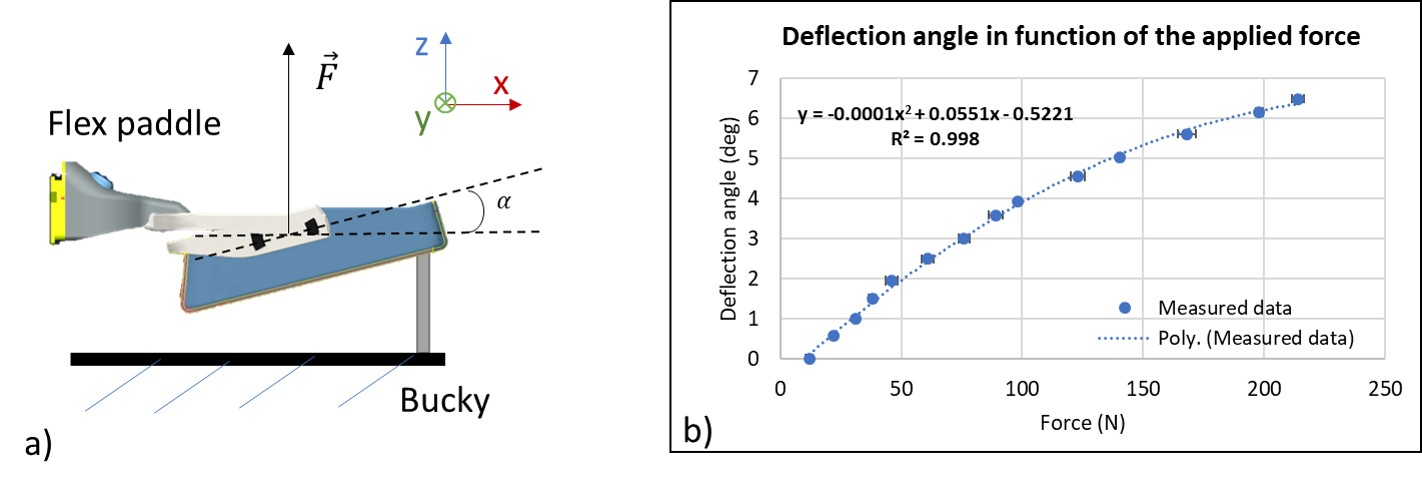
\includegraphics[width=0.9\textwidth,keepaspectratio]{figures/deflectionAngle.jpg} 
\caption{ a) Experiment set-up, b) Deflection angle in function on the applied force }\label{fig:deflectionangle}
\end{figure}

For the third paddle model, named the elastic paddle (EPM\nomenclature{EPM}{Elastic Paddle Model}), the deflection due to the materials properties are included. The paddle thickness is equal to $4mm$ and is made of Lexan material ($\lambda_{lexan}= 2,25*10^6 \ kPa$ and $\nu_{lexan}= 0.4$).   Only one translational degree of freedom in the downwards direction was considered. The paddle is modeled using shell elements. 

The interaction between the compression paddles and the breast was modelled using a frictionless contact. The penalty algorithm was used with a penetration factor equal to 0.1 and a contact stiffness equal to 1. 
 
\subsection{Breast compression mechanics}

The compression of a small breasts may be complex. Sometimes the technologist has to hold the breast between the image receptor and the paddle until the compression force is high enough to preclude breast from sliding outside of the compression area. These difficulties are also meet in a simulation framework, all the more so because the breast manipulation performed by the technologist is not reproduced. To facilitate the compression task, the following breast compression tests are performed only with the larger breast geometry.

In a clinical framework, woman breast is compressed only in an up-right or prone body position. When breast is compressed the gravity induced tissues pre-stresses can be neglected when compared to the compression induced stresses \citep{han_development_2012, ruiter_model_based_2006, sturgeon_finite_element_2016}.  Therefore, in this section, the prone breast configuration was used as reference configuration by neglecting the tissues internal pre-stresses dues to gravity loading. The breast compression is simulated using the rigid paddle model. 

Previously developed biomechanical model is implemented using the breast geometry of the second volunteer. Because of a large computation time, the constitutive parameters were not adapted to the volunteer-specific mechanical behaviour. Their values were taken from the literature \citep{han_nonlinear_2014,rajagopal_modelling_2007,gefen_mechanics_2007}, and are the following $\lambda_{breast}=0.5 kPa$, $\lambda_{muscle}= 10kPa$, $\lambda_{skin}=10$, $\lambda_{fascia}= 160kPa$.    

To simulate the cranio-caudal incidence, the image receptor is positioned at the inframammary ligament level while the paddle compresses the breast by a downward movement. The compression is stopped then the target breast thickness is reached. The target thickness is given by the data recorded during the volunteers last mammogram (Table \ref{tab:forceandthichnessdata}). The Figure \ref{fig:thicknessforcerelationNH} shows the breast thickness as function of the applied force for the flex and the rigid paddles. The breast thickness is considered constant and is equal to the distance between the image receptor and the paddle. 
 
\begin{figure}[!h]
\centering
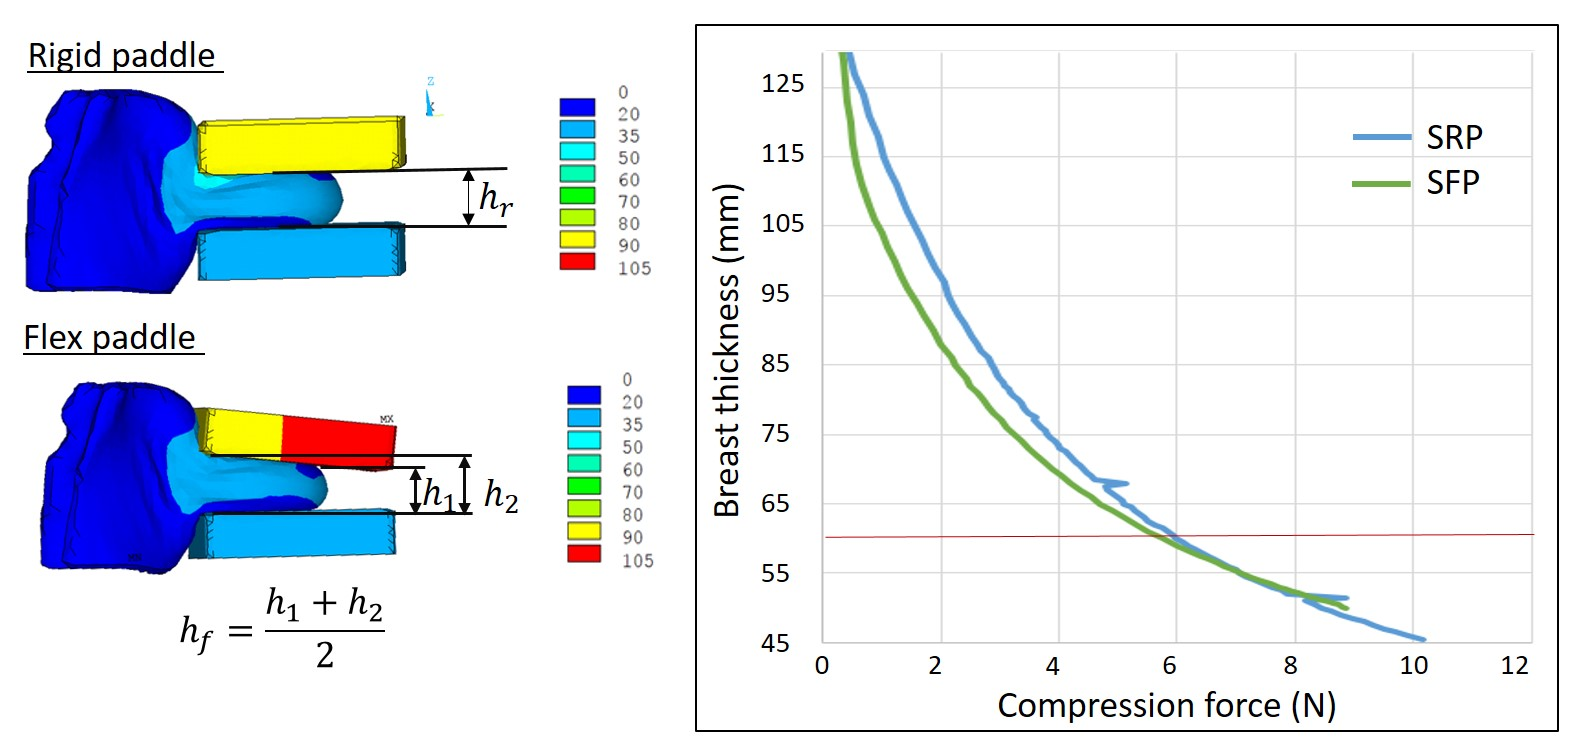
\includegraphics[width=0.9\textwidth,keepaspectratio]{figures/compressionforceNH.jpg} 
\caption{Breast flattening curve as function of the applied force for a Neo-Hookean strain energy function. SRP - standard rigid paddle, SFP -standard flex paddle}\label{fig:thicknessforcerelationNH}
\end{figure}

One can see that, the total compression force at the target breast thickness ($50mm$) is about 10 times lower when the force measured during the volunteer's last mammography ($6N$ versus $94.8N$). Even if the used constitutive models are not adapted to the patient mechanical properties, a force of $6N$ remains too low when compared to the standard compression force of $120N$ \citep{chida_reduced_2009}.   Several compressions were tested (paddle closer to the juxtathoracic area, frictional contact with different friction coefficient) without observing any significant increase of the compression force. 

An analysis of the literature revealed that the constitutive parameters used for modelling the breast compression are higher than the ones used for modelling the breast deformation under gravity loading.  \cite{sturgeon_finite_element_2016} have estimated the tissues deformation under compression considering the initial shear modulus for a Neo-Hookean strain energy function to $\mu_{skin} = 88kPa$, $\mu_{adipose} = 1kPa$ and $\mu_{glandular}= 10kPa$. Moreover, within simulation the obtaned compression force versus breast thickness relation does not show an asymptotic behaviour as described by \cite{de_pain_2015}.  Therefore, one can conclude that, for high strains, the soft tissues undergo a stiffening process more rapidly than may be described by a Neo-Hookean law.

The limitations of the Neo-Hookean model to capture the mechanical response of some nonlinear materials is well known \citep{kaliske_finite_1997}. For large strain rates, the Neo-Hookean material may undergo a relaxation and therefore becomes easier to deform. Therefore, different strain energy models have to be considered for breast compression modelling.

\subsubsection*{Gent energy function}

The Gent energy distribution function (see Section \ref{subsection:constitutivemodels}.a)  can be used as an alternative for modelling the soft tissues mechanical response. This model is characterized by three parameters ($\mu$, $K$, and $J_m$). When $J_m \longrightarrow \infty$, the Gent model is reduced to the Neo-Hookean model (Figure \ref{fig:GentvsNeoStrain}.a). Moreover, \citep{chagnon_comparison_2004} have showed that, for small deformations, the Gent model is equivalent to the Neo-Hookean one regardless the $J_m$ value. The $J_m$ acts as a stiffening parameter and define the upper limit of the first invariant of the left Cauchy-Green deformation tensor (Figure \ref{fig:GentvsNeoStrain}.a). 
 
\begin{figure}[!h]
\centering
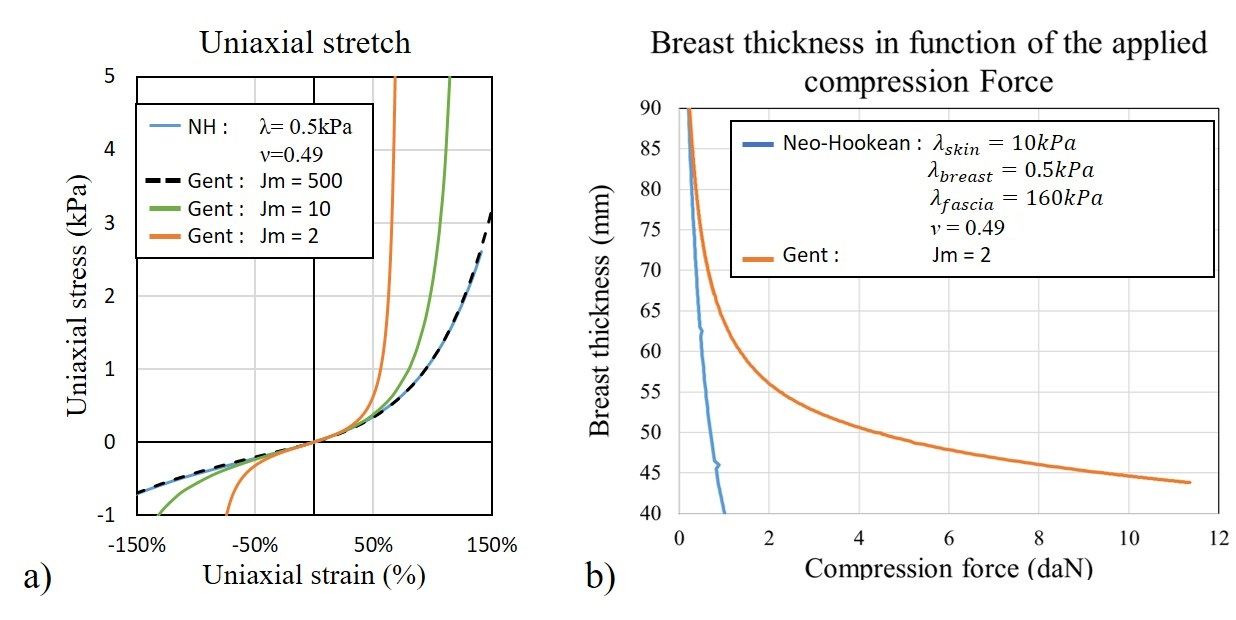
\includegraphics[width=1\textwidth,keepaspectratio]{figures/GentvsNeoStrain.jpg} 
\caption{a) Stress-strain relation for Neo-Hookean and Gent energy function; b) Breast flattening curve as function of the applied force for a Gent energy function.}
\label{fig:GentvsNeoStrain}
\end{figure}

These properties are particularly interesting for our simulation framework. In the previous chapter the material properties have been estimated and validated for multi-loading gravity simulations. Knowing that, the strain range due to gravity loading is smaller than the one due to breast compression. The $J_m$ parameter may be estimated such that, for relative small strain, the Gent model will be equivalent to the Neo-Hookean model; however for larger strain  the energy function will behave asymptotically in order to approach a compression force equivalent to the standard compression force (Figure \ref{fig:GentvsNeoStrain}.b). In such case, only the third parameter of the energy function have to be estimated ($J_m$), assuming that the initial shear modulus ($\mu$) and Bulk modulus ($K$) are already known from the multi-loading gravity optimization process.

Figure \ref{fig:GentvsNeoStrain}.b shows the breast flattening curve as function of the applied force for Neo-Hookean and Gent models. One can see that, then using the Gent form the curve behaviour is closer to the ones described by \cite{de_pain_2015}.

\subsection{Updated material constitutive models}

To compute tissues deformation under compression, the Gent energy function was used. The compression simulations were performed only on the right breast of both volunteers. The mechanical tissues properties of the first volunteer are set to the values obtained in the previous chapter ($\lambda_{breast}^r=0.3 kPa$, $\lambda_{skin}=4 kPa$, $\lambda_{fascia}=120 kPa$). As the optimization process was not performed for the second volunteer, the mechanical tissues properties are set to the values found in the literature ($\lambda_{breast}=0.5 kPa$, $\lambda_{muscle}= 10kPa$, $\lambda_{skin}=10$, $\lambda_{fascia}= 160kPa$).  

Several compression simulations using the standard rigid paddle were performed to determine the third parameter $J_m$. The chosen value is the one resulting in a force-thickness relation passing through the point defined in Table \ref{tab:forceandthichnessdata}. For the first volunteer, a breast thickness of $46mm$ with a compression force of $22N$ is obtained when $J_m = 1$. For the second volunteer, a breast thickness of $48mm$ for a compression force of $95N$ is obtained when $J_m = 2$. Because of convergence difficulties the Poison ratio for these simulations was set to $0.499$.

Figure \ref{fig:forceThicknessResults} shows the breast flattening curve as function of the applied force obtained with rigid and flex paddle models. All the simulations were performed with the Gent model of the strain energy distribution function. 

\begin{figure}[!h]
\centering
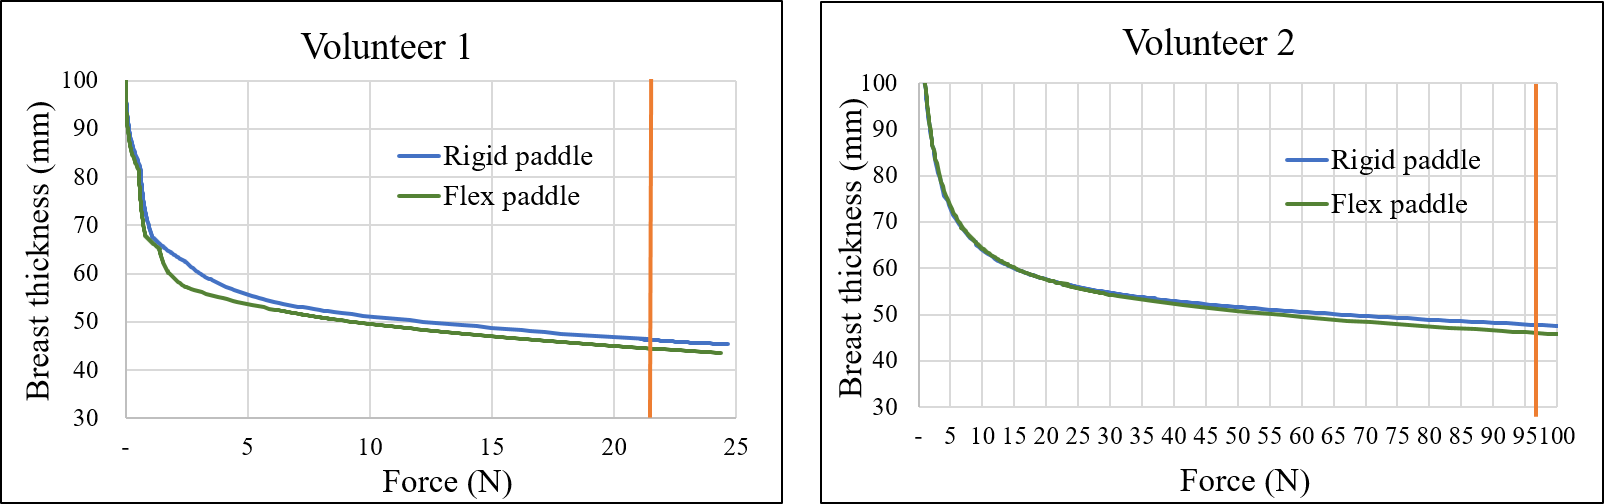
\includegraphics[width=1\textwidth,keepaspectratio]{figures/forceThicknessResults.png} 
\caption{Resulting breast flattening curve as function of the compression force with Gent constitutive model. }\label{fig:forceThicknessResults}
\end{figure}
    
\section{Simulation of digital images }
Digital mammography images of the compressed breast were simulated using the CatSim simulation environment \citep{de_low_2014,de_catsim_2007}. 


\begin{figure}[!h]
\centering
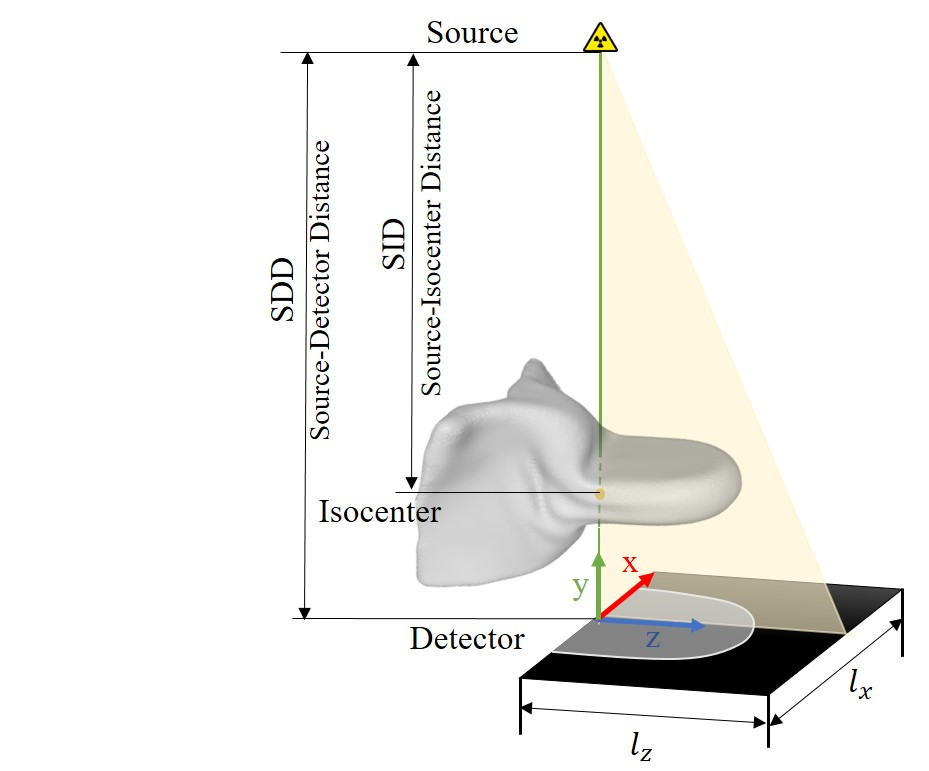
\includegraphics[width=0.65\textwidth,keepaspectratio]{figures/systemgeometry.jpg} 
\caption{A schematic illustration og the simulated GE Senographe Pristina TM mammography unit.}
\label{fig:systemgeometry}
\end{figure}
%SDD = 660mm, SID = 636.76


\subsection{Physical characteristics}
The X-rays projections of phantom objects were simulated using a GE Senographe Pristina-like system topology (Figure \ref{fig:systemgeometry}). The focal spot was modelled as a point source. A 24 keV mono-energetic x-ray beam was considered.  This beam quality is similar to the effective x-ray energy of a 34 kVp Rhodium (Rh)/Silver (Ag) target/filter) spectrum filtered by a 46 mm compressed breast. Spreading of the light photons in the CsI scintillator of the detector was modelled by filtering the detected x-ray beam by an empirically assessed modulation transfer function of the CsI scintillator. X-ray scatter from the test object and other system components were not included in the simulation. Only quantum noise, modelled by a Poison random distribution, was considered as noise source. The simulated x-ray flux was tuned to match the average signal intensity ($\langle SI \rangle$) and signal-to-noise ratio (SNR) measured in real images of a 46-mm thick 20\% fibroglandular equivalent phantom acquired with the automatic optimization of parameter mode. To do so, a calibration was performed on a real PRISTINA mammography unit. 

\subsection{Breast phantom objects}

The phantoms were created by first extracting the compressed breast other shape. Then, a set of microcalcifications were inserted into each compressed breast volume. The smallest breast volume contains 21 microcalcifications arranged in a matrix of 7 rows and 3 columns (Figure \ref{fig:microcalcifications}.a). The largest breast volume contains 56 microcalcifications arranged in a matrix of 7 rows and 8 columns. The matrix of calcifications is parallel with the entrance surface of the image receptor and positioned at the breast mid thickness (Figure \ref{fig:microcalcifications}.b). The distance between two consecutive columns or rows is equal to 10mm. The anatomical background was assumed to be a uniform breast-equivalent material composed of glandular/adipose tissue with a 20/80 ratio. Two simulations were performed for each compression considering $\mu calc$ of 0.2 mm and 0.3mm in diameter.

\begin{figure}[!h]
\centering
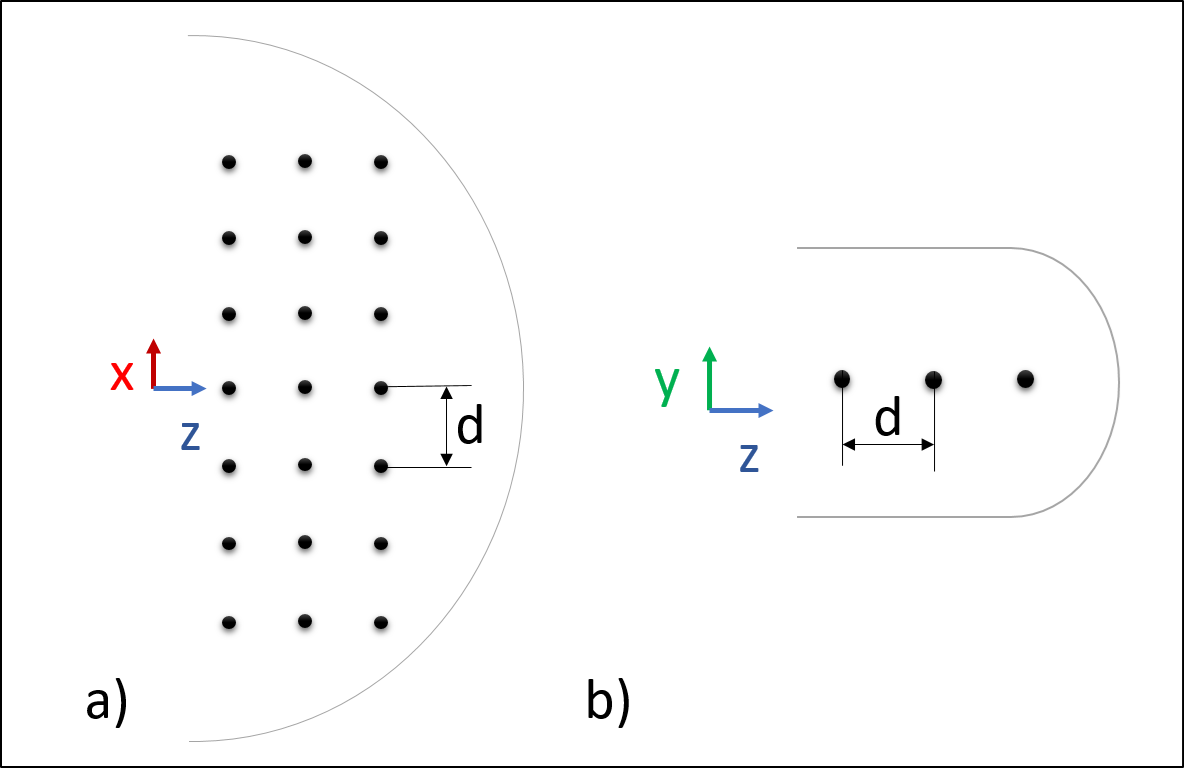
\includegraphics[width=0.5\textwidth,keepaspectratio]{figures/microcalcifications.png} 
\caption{Microclcification distribution over the smallest breast volume $(d=10mm)$: a)axial view, b) sagittal view.}\label{fig:microcalcifications}
\end{figure}


Microcalcifications $(\mu calc)$ were simulated as round-shaped surface mesh. To add irregularities, initially spherical objects were randomly deformed. Their with X-ray attenuation properties correspond to the attenuation of aluminium (Al) at 24 $keV$ and with a volumetric mass density corresponding to 60\% of the Al density, i.e. 1.63 $\frac{kg}{m^3}$.  The choice of 24 $keV$ corresponded to the photon energy of the x-ray source used in our study. 



\section{Compression quality metrics}\label{section:compressionqualitymetrics}

The measures used to quantify the three criteria characterizing the quality of breast compression (patient comfort, image quality and average glandular dose) are described in the following section.  

\subsection{Patient comfort}

Today, the pain estimation and quantification still remain an open question. During mammography, the perceived pain, or its interpretation, may depend on the social status, pain history or psychological condition of the patient. But can also depend on the physical parameters as the compression force, amount of deformation or pressure on the skin surface. In clinical studies, the patient comfort is assessed using pain scales. The repeatability of such methods is questionable, because they are based on the patient own interpretation and expertise. More quantitative measures such as pupil dilatation, heart rate are interesting in assessing the patient comfort, however they may indicate not only the pain but also the fear of pain.        

In this work, only the physical pain associated with tissues deformation was considered. In this scope, the maximal stain and stress intensities as well as the maximal pressure intensity at the contact surface between the breast and the compression paddle were chosen as pain quantifiers. Their distribution over the breast volume were obtained from FE simulation of breast compression and were analysed in order to compare the patient experience between two distinct compressions. 

\subsection{Image quality }\label{section:averagegalndulardose}
 To assess the image quality the signal-difference-to noise ratio (SDNR \nomenclature{SDNR}{Signal Difference to Noise Ratio}) per pixel of the inserted microcalcifications was measured in the raw projection images. Squared ROIs of $1cm \times 1cm$ centred on the $\mu calcs$ position were defined to compute the average detected signal per background pixel $\langle SI_{back}\rangle$ and the standard deviation in the background signal intensity $\sigma_{back}$. The SDNR is defined as follows
 \begin{equation}
 SDNR = \frac{\langle SI_{back}\rangle - \langle SI_{\mu calc}\rangle}{\sigma_{back}},
\end{equation}

 
Additionally, the SNR was computed using the same ROIs as follows  
 \begin{equation}
 SNR = \frac{\langle SI_{back}\rangle}{\sigma_{back}}.
\end{equation}



\subsection{Average glandular dose}
The estimation of breast dose remains an essential component of quality control for x-ray mammography. In this section, the average glandular dose was derived using the approach proposed by \cite{dance_additional_2000} regardless the paddle type. The method uses conversion factors to relate measurements of the incident air kerma $K$ at the upper surface of the breast to the mean dose to the glandular tissue within the breast. 

\begin{equation}
AGD = K g c s
\end{equation}

Were g and s are conversion factors giving the AGD in function of the target/filter combination and breast thickness (range between 20-110mm) for a breast granularity of 50\%. The factor c extends the AGD estimation for different breast granularity. Monte-Carlo simulation were used for the estimation of these factor by modelling the compressed breast by a semi-circular cross section cylinder. 

The numerical phantom is characterized by a uniform thickness, however a mammography compression implies variable breast thickness due to paddle elasticity (SRP) and paddle flexibility (SFP). In a clinical framework, the breast thickness is adjusted by applying an offset characterizing the paddle deflection during compression.      

As the paddles elasticity is neglected, the AGD for a rigid paddle is computes by assuming that the breast thickness is equal to the distance between the image receptor and the paddle itself. Regarding the flex paddle, the breast thickness decreases quasi-linearly from the chest wall to the nipple. Thus, the breast thickness was computed as the mean of the maximal and minimal distance from the image receptor to the compression paddle.

\section{Results}\label{section:breastcompressionevaluation}
Two studies were performed using the previously defined components for modelling the breast compression and simulating digital mammography. First, the results of a comparative study between flex and rigid paddles is presented where the image quality, AGD and patient comport are addressed. Next the impact of breast positioning on breast mechanics is analysed.   
\subsection{Compression quality for rigid and flex paddles}

To compare the breast compression quality when using a SFP against a SRP, the rigid and flex paddle models are used. The right breast of the two volumes is first compressed until the target breast thickness is obtained (Table \ref{tab:forceandthichnessdata}). Then the breast phantoms with $\mu calc $ are imported into CatSim environment and mammography images are simulated.

The resulting breast thickness after compression vary by less than $2mm$ between rigid and flex paddle for both volunteers (Table \ref{fig:table_compression_results}). Accordingly, no significant difference was found between the estimated AGD, while a dose reduction of $2\%$ for the smaller breast and $4\%$ for larger breast was observed.

\begin{figure}[!h]
\centering
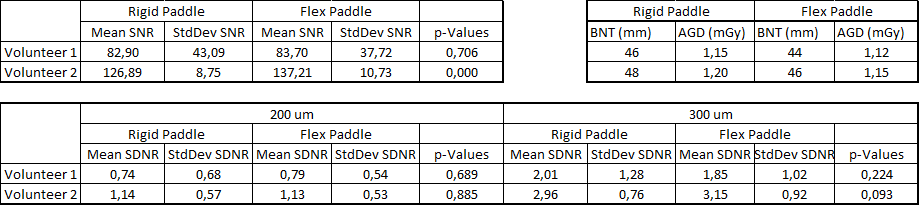
\includegraphics[width=\textwidth,keepaspectratio]{figures/table_compression_results.png} 
\caption{Breast nominal thickness (BNT), average glandular dose (AGD), signal-to-noise-ratio (SNR) and signal-difference-to-noise (SDNR) for both volunteers and both compression paddle types}\label{fig:table_compression_results}
\end{figure}

The SNR and SDNR have been estimated and compared between flex and rigid paddles. When using a flex paddle instead of a rigid paddle on the largest breast (volunteer 2), we observe a statistically significantly higher SNR. The same trend is observed on SDNR for both 200 and 300 µm microcalcifications, while not statistically significant. We did not observe any statistically significant difference in SNR or SDNR for microcalcification of any size when considering the compression of the smallest breast by a rigid or a flex paddle. Therefore, despite a breast thickness varying linearly from chest wall to nipple when the flex compression paddle is used, the image quality is preserved or improves compared to the image quality obtained with the rigid compression paddle.

In a clinical study, \cite{broeders_comparison_2015} have also compared the image quality and patient comfort between the standard rigid and flex paddles. According to the authors, the standard flex paddle performed slightly better image quality in the projected breast area, however it moved breast tissue from the image area at chest wall side. According to our compression simulation, for the small breast volume, no difference in tissues lateral displacement was observed. On the other hand, for the larger breast, using the flex paddle have indeed increased the tissues displacement toward the chest wall side , but not by more than $4 \ mm$ (Figure \ref{fig:rigid_flex_y_displacement}).  

\begin{figure}[!h]
\centering
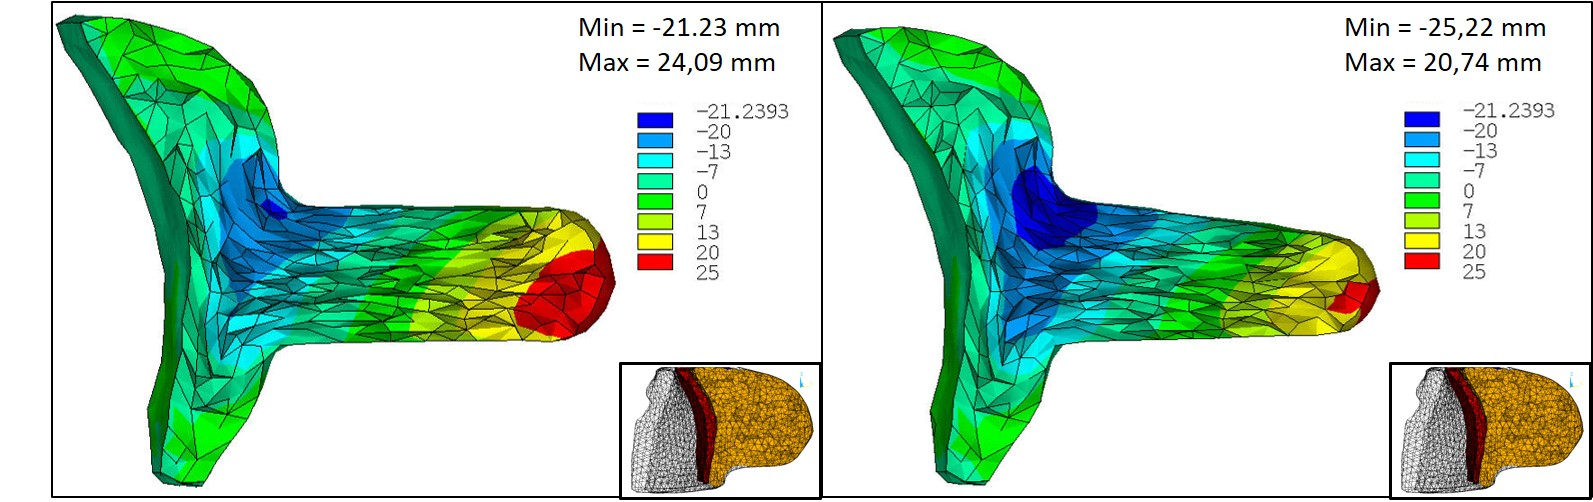
\includegraphics[width=1\textwidth,keepaspectratio]{figures/rigid_flex_y_displacement.jpg} 
\caption{Node displacements on the direction paralele to the paddle (Oy axsys).}\label{fig:rigid_flex_y_displacement}
\end{figure}

The resulting internal stress and strain distributions, as well as contact pressure maps were derived at compressive forces of 22 N for the first volunteer (Figure \ref{fig:subject1_compressionResults}) and 95 N for the second one (Figure \ref{fig:subject2_compressionResults})

\begin{figure}[h]
\centering
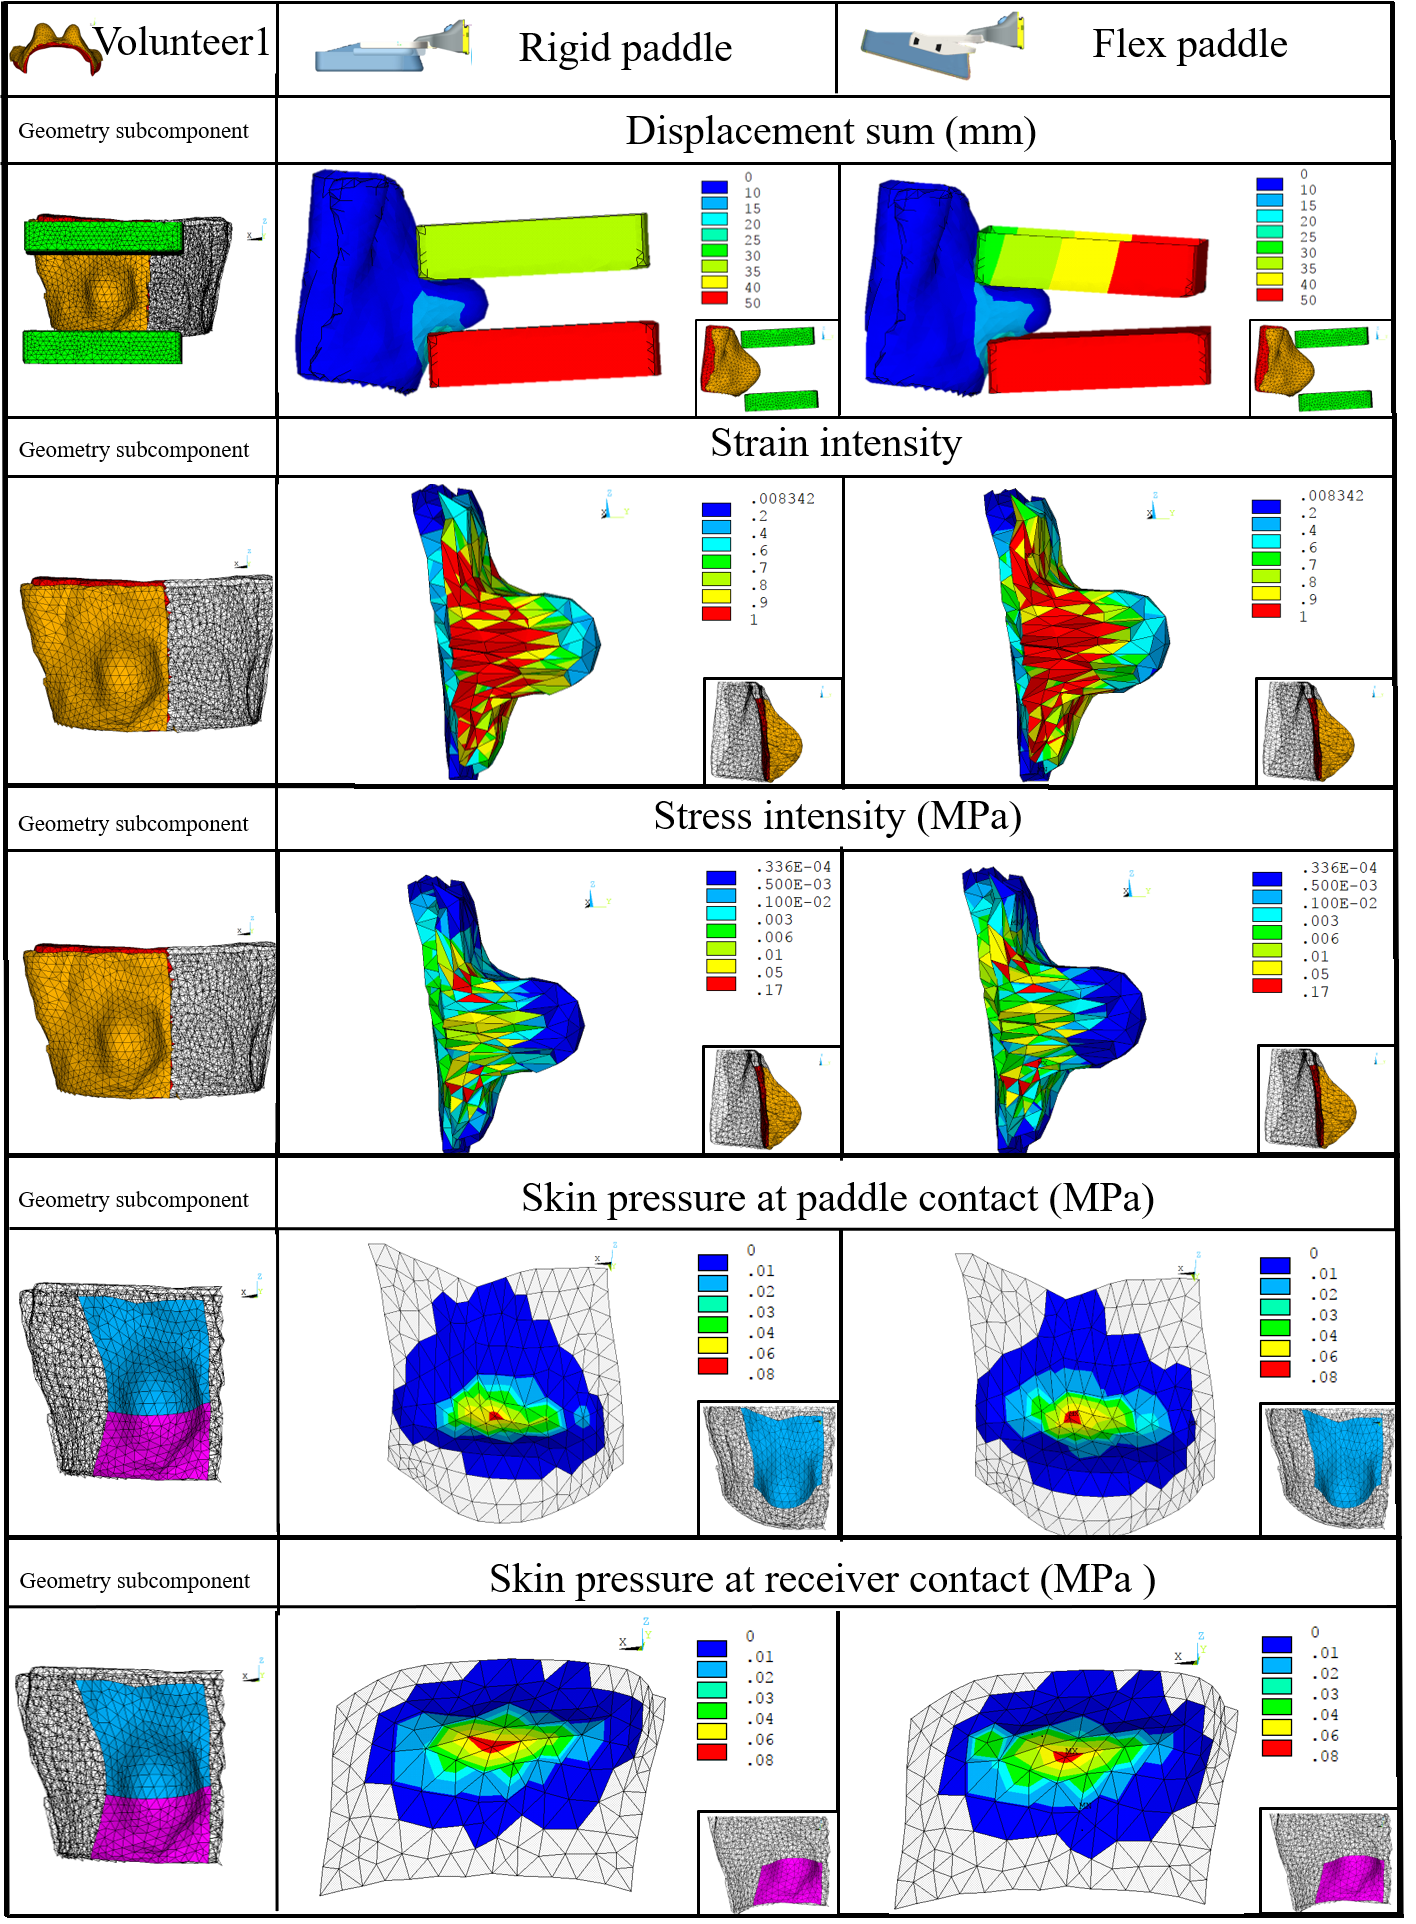
\includegraphics[width=0.95\textwidth,keepaspectratio]{figures/subject1_compressionResults.png} 
\caption{Stress, strain and contact pressure distribution for the first subject}\label{fig:subject1_compressionResults}
\end{figure}

\begin{figure}[h]
\centering
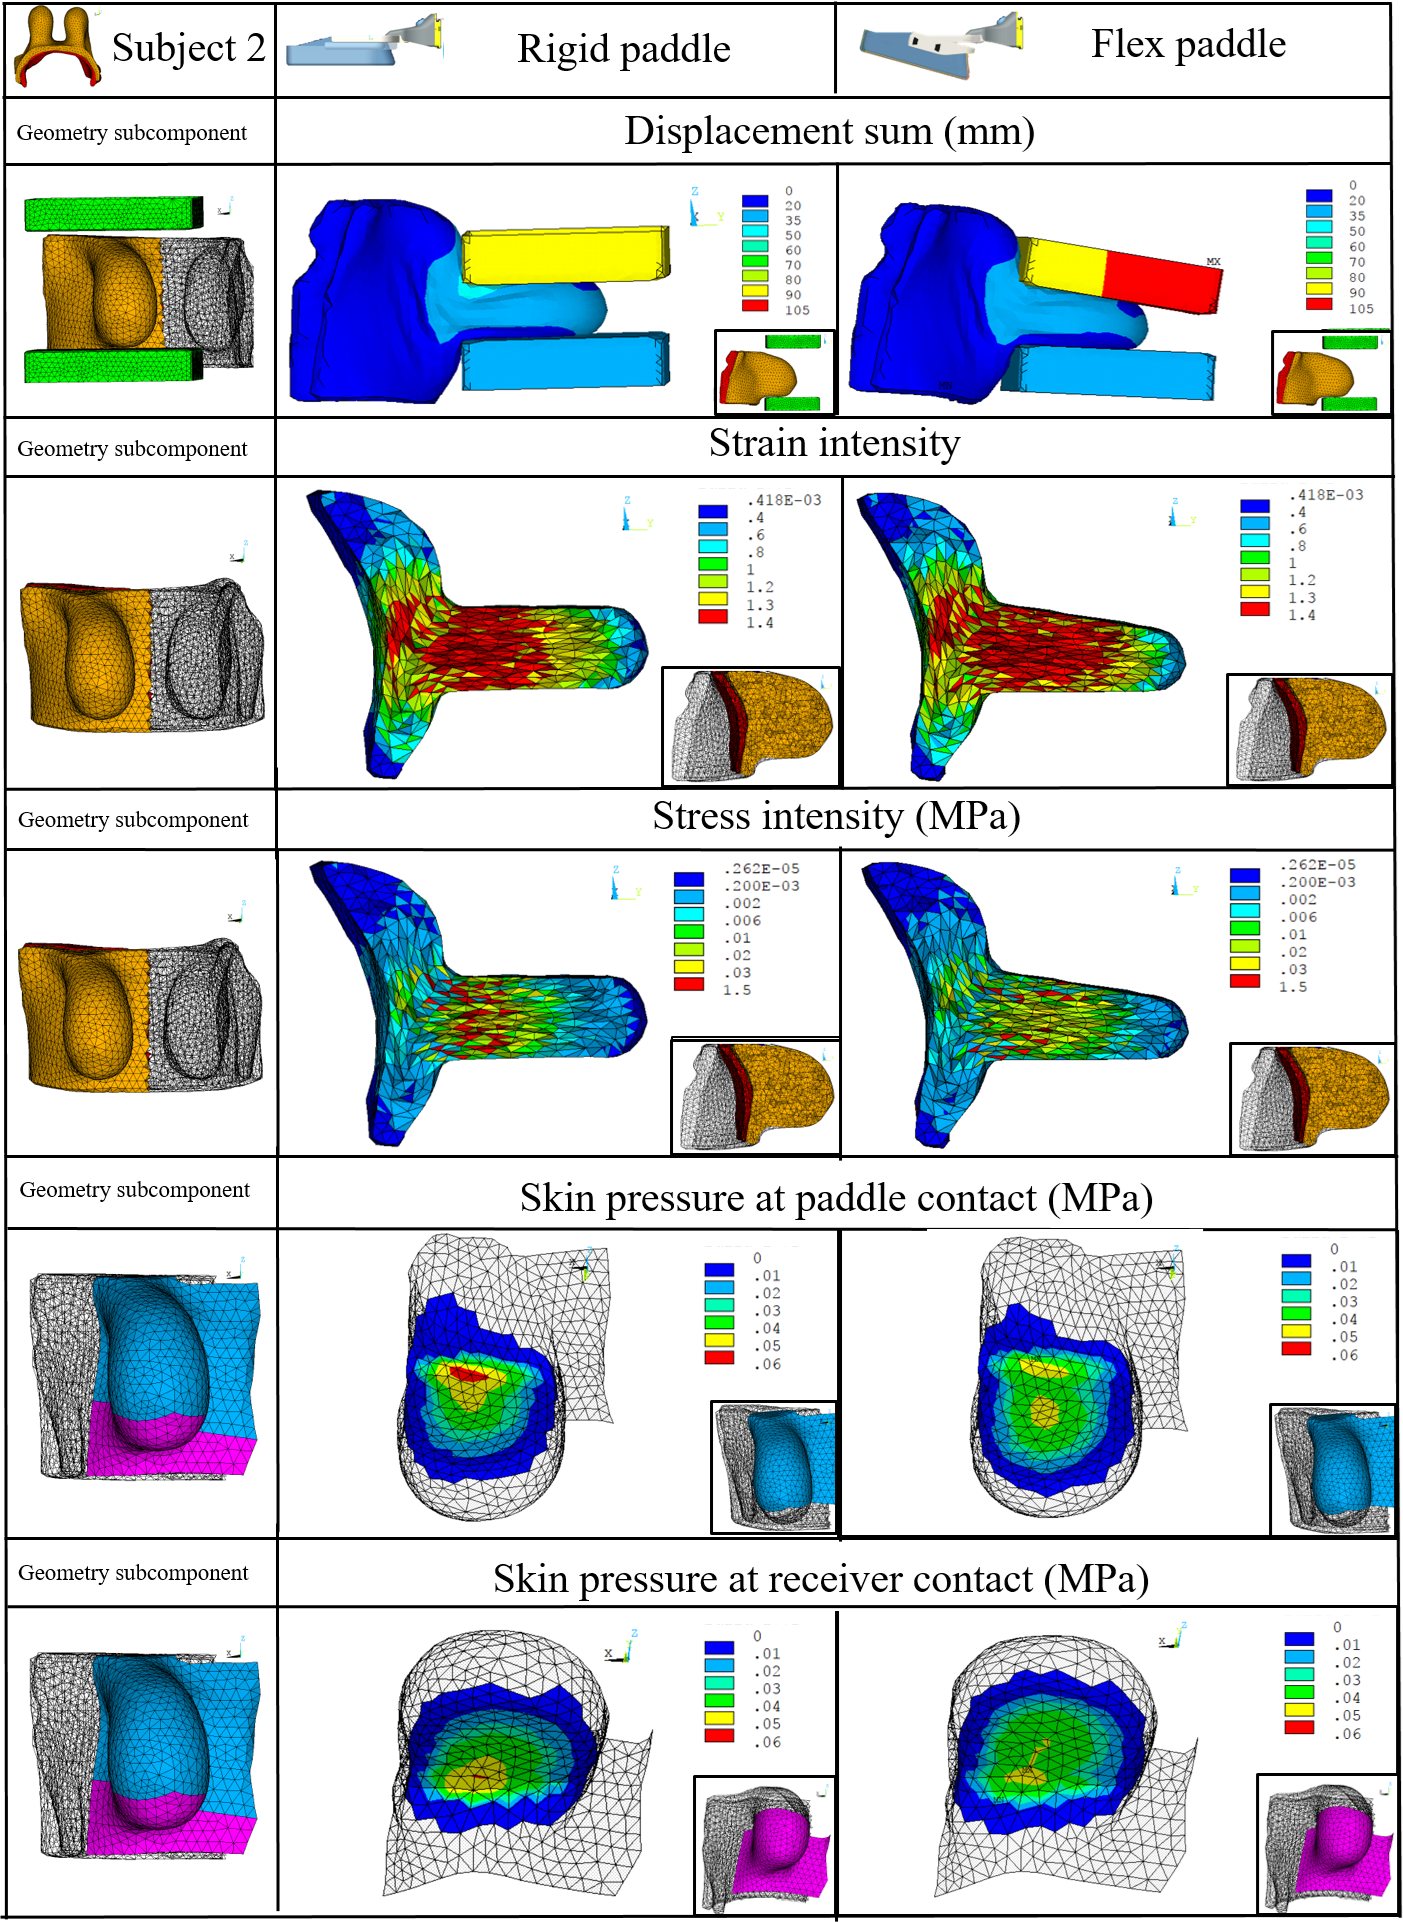
\includegraphics[width=0.95\textwidth,keepaspectratio]{figures/subject2_compressionResults.png} 
\caption{Stress, strain and contact pressure distribution for the second subject}\label{fig:subject2_compressionResults}
\end{figure}


As concerns the small breast volume (Figure \ref{fig:subject1_compressionResults}), there is no significant difference between FPM and RPM in pressure distribution over the skin surface or in internal stress/strain intensity distributions. For both compression paddles, high pressure at the skin surface is concentrated in the juxtathoracic region with a maximum pressure of 77.7 kPa. In addition, the FE simulations confirm that in small breasts the paddle tilt is too small to impact the tissues compression in the middle part of the breast. 
FPM applied on large breast volumes (Figure \ref{fig:subject2_compressionResults}) results in significantly lower intensities of pressure at the skin surface in contact with the compression paddle, with a maximal pressure of 37 kPa, compared to 56 kPa when using RPM. No significant difference in the measured maximal intensities of strain and stress was observed, however strain and stress distribution patterns are different. When the breast is compressed with a rigid paddle, maximal strain and stress are concentrated in the retromammary space and decrease considerably toward the nipple. When a flex paddle is used, stress and strain are more uniformly distributed over the breast volume with the highest values in the middle third of the breast.

\clearpage
The areal pressure distribution patterns have already been demonstrated in the work by \cite{dustler_breast_2012}. The authors have studied the pressure distribution patterns of 103 women undergoing breast compression with a rigid paddle at different compression levels. Four groups have been differentiated: a) skin pressure widespread over the breast (29\%); b) skin pressure concentrated on the central part of the breast (8\%); c) skin pressure concentrated on the juxtathoracic region (16\%); d) skin pressure concentrated along a narrow zone at the juxtathoracic region (26\%).  The pressure distribution patterns observed for our first and second volunteers correspond to the group d and a respectively.


\subsection{Breast positioning impact on compression mechanics}\label{subsection:breastpositioning}

The breast positioning impact on compression mechanics was assessed using the elastic paddle model. The right breast of the geometry from the second volunteer was compressed with different paddle position with respect to the thoracic cage (thoracic cage to paddle distance TPD). The breast was compressed until a minimal thickness of $50mm$ is reached. Then, the compression force as well as surface pressure at the contact with the compression paddle were compared. The compression force was computed as the product between the mean surface pressure and the contact area $\langle P_{contact}\rangle \ast  A_{contact}$.

Figure \ref{fig:elasticpaddle} shows the strain/stress as well as the pressure distributions over the contact area for three  distinct distances between the paddle and the thoracic cage. The compression force varies considerably within paddle positions. A compression force of $59\ N$, $94\ N$ and $158\ N$ was obtained when the paddle was positioned at a distance from the chest wall of $48\  mm$, $40\  mm$ and $33\ mm$ respectively. Only with $15\ mm$ closer to the chest wall the force intensity was tripled. 
 
\begin{figure}[!h]
\centering
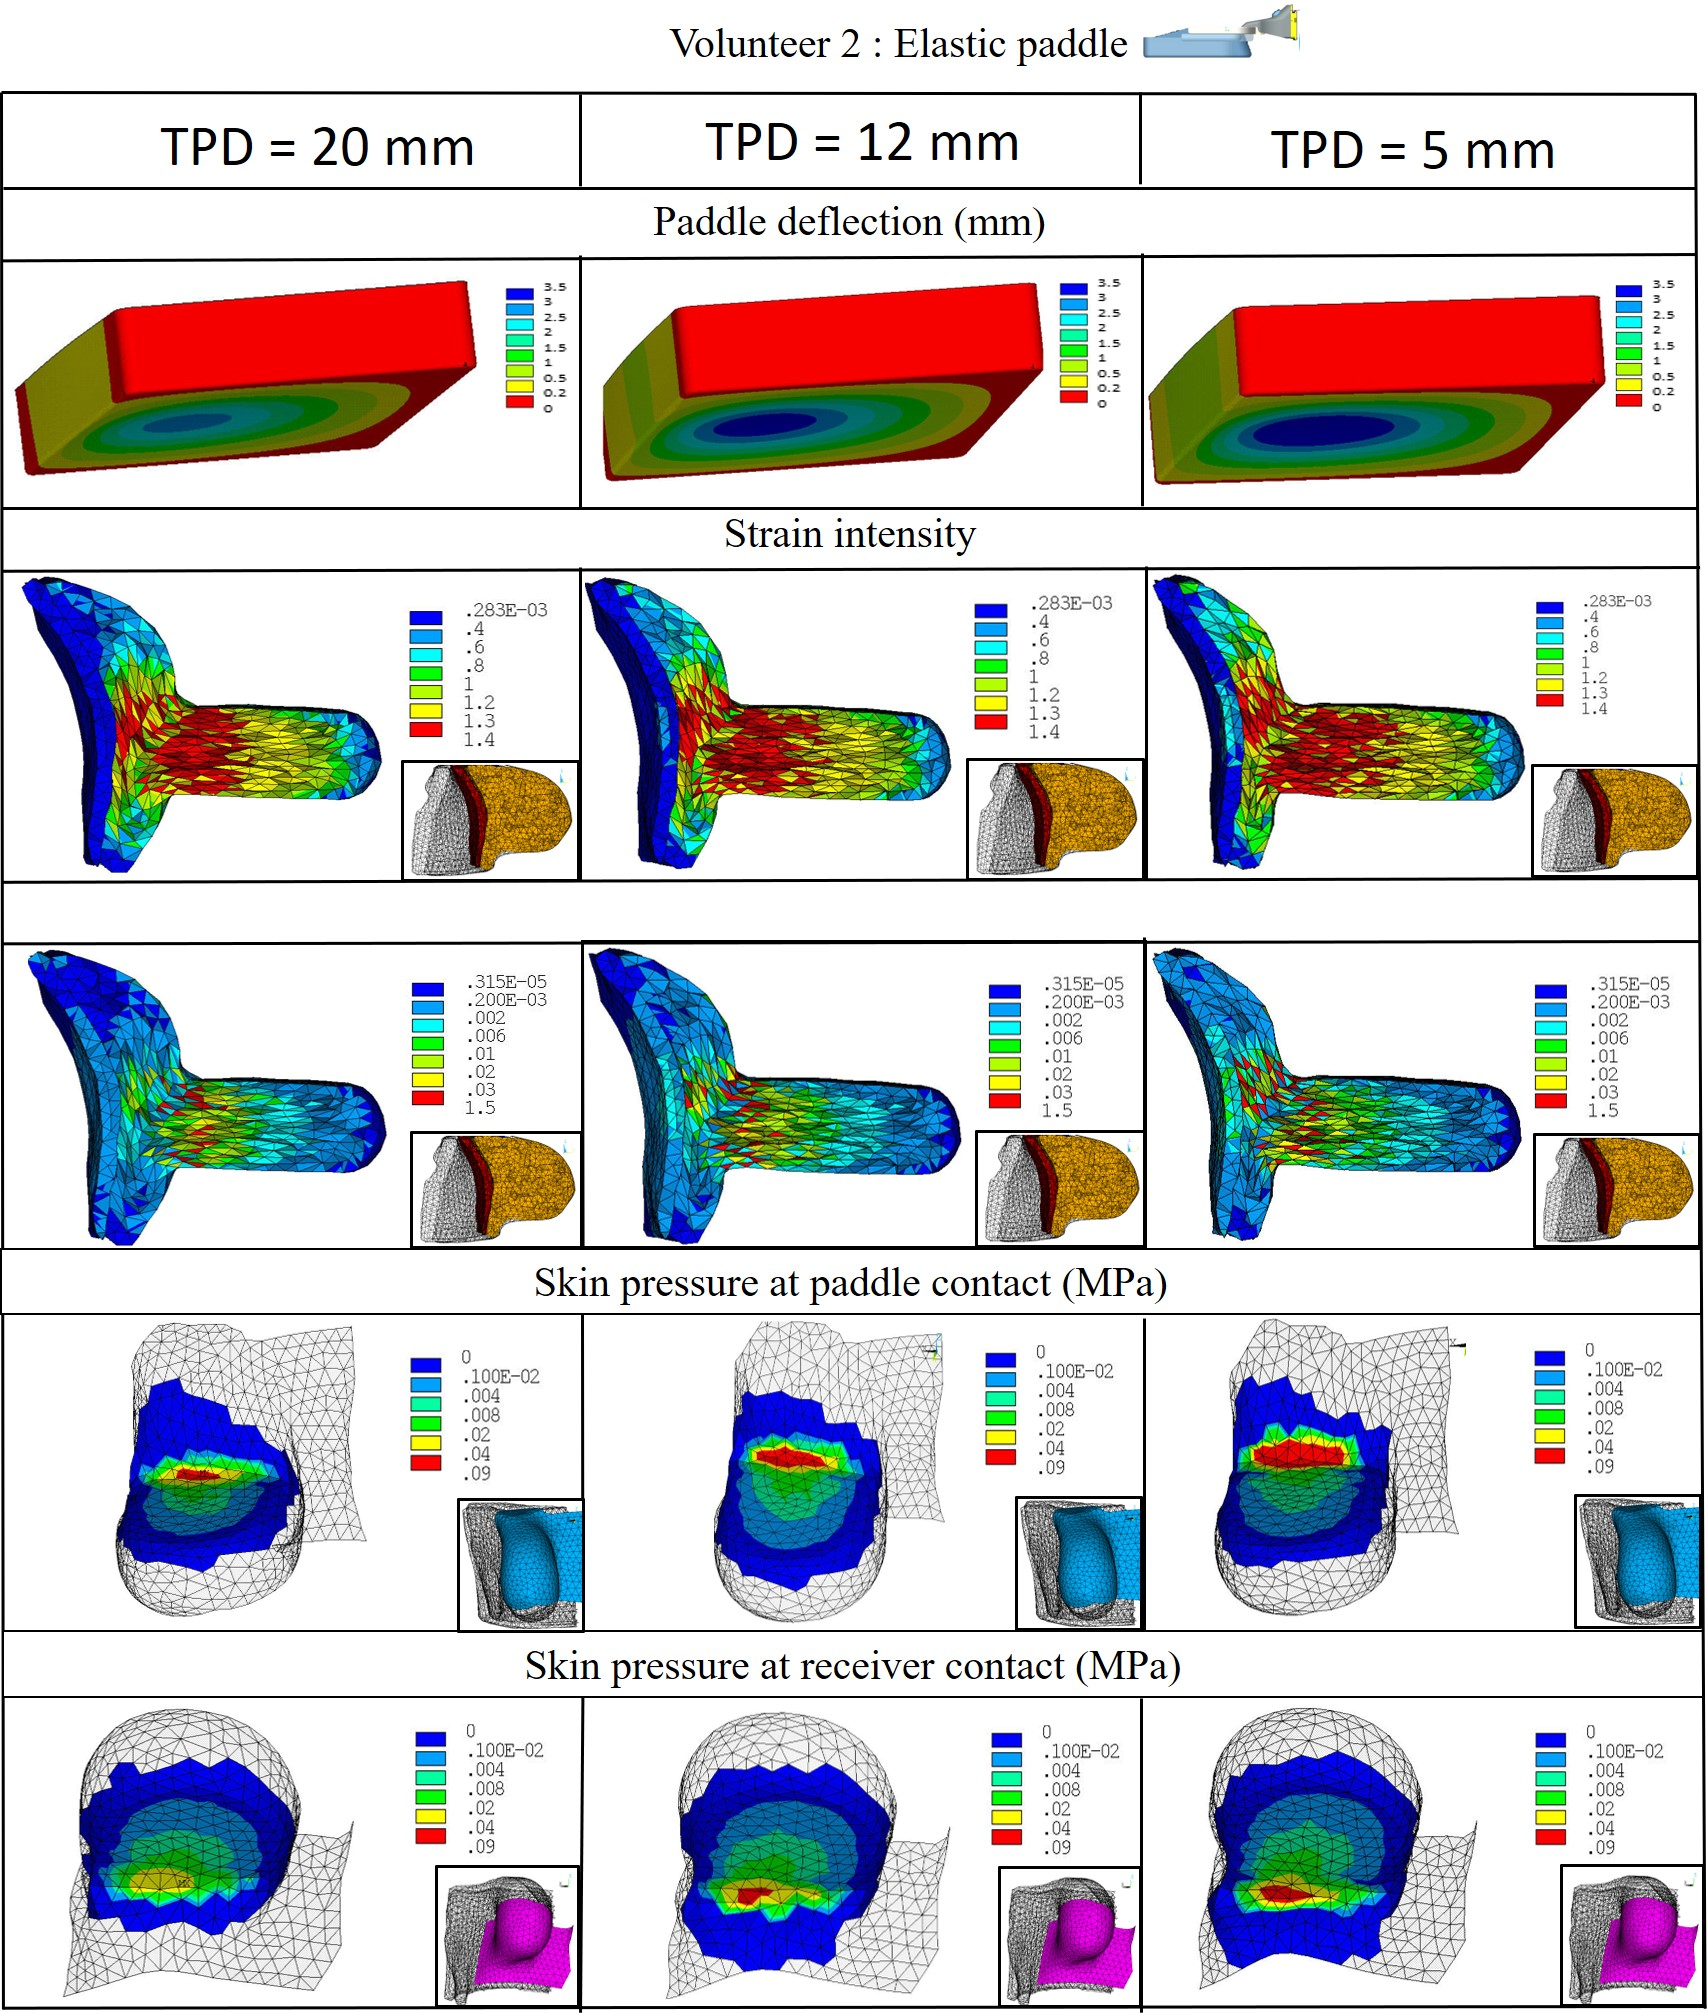
\includegraphics[width=1\textwidth,keepaspectratio]{figures/elasticpaddleresults.jpg} 
\caption{Stress, strain and contact pressure distribution for a variable thoracic cage to paddle distance (TPD).}\label{fig:elasticpaddle}
\end{figure}


Because of the paddle elasticity the breast thickness varies slightly with a maximal deflection equal to $3.5\ mm$ (Figure \ref{fig:elasticpaddle} first line). A very small difference between the maximal paddle deflection was observed within the previous three compressions   $(\sim 1\ mm)$, thus the image quality or AGD were not significantly impacted by the thickness variation. However, wider is the space between the chest wall and the compression paddle, fewer clinically relevant tissues are included in the projected mammography image. In a standard framework the radiologist will include as much as possible of breast soft tissues in order to reduce the risk of missing a suspicious lesion.

When looking to the stain distribution, one can see that, when the compression paddle is positioned closer to the chest wall, the juxtathoracic soft tissues undergo higher deformation resulting also in a higher stress intensity. Concerning the skin surface pressure distribution, the highest intensities $ (\sim 90\ kPa)$ are always concentrates in the juxtathoracic area. However, for a thorax to paddle distance equal to $33\ mm$, the area corresponding to the high pressure is considerably larger. This means that, a good part of the total force was  namely used to compress the tissues in the juxtathoracic area only, which may increase the patient discomfort.

\section{Discussions and conclusion}\label{section:compressionfem:conclusion}

In this chapter, the breast compression was simulated using three paddles models, the rigid, flex and elastic models. In order to comply with the compression mechanics as described in literature, an update of the tissues constitutive models was needed. Appling the Gent form of strain-energy potential, instead of the Neo-Hookean form, allowed to obtain compression force magnitudes comparable with the real subject data.  
However, this estimation does not characterize the patients-specific mechanical properties and gives only an estimation of a standard behaviour.  The second experiment shows that, to obtain a proper estimation of the $J_m$ parameter, more information as paddle position with respect to the breast volume is needed. 

The patient comfort (measured as strain and stress) as well as the image quality (measured as SNR, SDNR ) and AGD were compared for breast compression with rigid and flex paddles. The results from the two volunteers have been analysed. The compression simulations indicate that, for the smallest breast, there is no significant difference for the patient perceived pain when using the rigid or the flex paddles. We did not observe any statistically significant difference in SNR or SDNR for microcalcification of any size. Therefore, our results suggest that using a flex paddle should not significantly impact image quality and delivered dose in small breasts and should not reduce significantly the perceived pain.   
For the largest breast, our simulations indicate that using a flex paddle may reduce the maximal pressure intensity on the skin surface by about 30\% compared to the rigid paddle. The tissues deformation is more uniformly distributed inside the breast volume, and the highest deformation occurs in the middle breast region corresponding to the supposed location of dense tissues. Moreover, our simulations have shown that flex paddle have no significant impact on the average glandular dose and improves image quality compared to the rigid paddle. However, the breast compression with flex paddle is suspected to facilitate the displacement of the fibroglandular tissues into the retromammary area. As the breast thickness increase linearly from the nipple to the chest wall, the retromammary area is characterized by a low image quality. 


The impact of breast positioning on patient comfort and image quality was also addressed. Three paddle positions with respect to the chest wall were studied using the elastic compression paddle. Even if a variable breast thickness is obtained due to the paddles deflection, the variations are too small ($\sim 1mm$) to impact the AGD or the resulting image quality in terms of the SNR or SDNR. However, by excluding the retromammary tissues, information on small posterior cancerous legions may be lost. In terms of patient comfort, the simulations have shown that the high pressure are always localized in the juxtathoracic areas. When the paddle is too close to the chest wall, the compression force is mostly dissipated on this narrow area resulting in very high pressures compared to the skin pressure over the breast ($90kPa\ vs\ 10kPa$).
